\documentclass{standalone}
\usepackage{tikz}

\begin{document}
	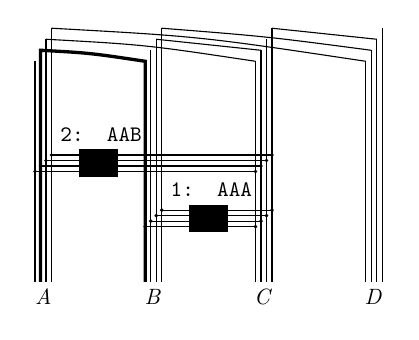
\begin{tikzpicture}[scale=0.7, every node/.style={scale=0.8}]
		%Säulen
		\foreach \i in {0,2,4,6} {
			\foreach \j in {0,0.1,0.2,0.3} {
				\draw[thin] (\i+\j,1) -- (\i+\j,5+\j*2);
			}
			\node[below] at (\i+0.15, 1) {\emph{\char\numexpr65+\i/2}};
		}
		%		\draw[very thick] (2.2,1) -- (2.2,5.4);
		
		%		\draw[thin](0,9) .. controls (1,9.05) .. (2,9);
		
		%Querverbindungen
		\foreach \j in {0.1,0.2,0.3} {
			\draw[thin](\j,5+\j*2) .. controls (\j*10,5+\j*1.5) .. (\j*20,5);
		}	
		\draw[very thick] (0.1,1) -- (0.1,5.2) .. controls (1,5 + 0.1 * 1.5) .. (2,5) -- (2, 1);
		
		\foreach \j in {0.2, 0.3} {
			\draw[thin](\j+2,5+\j*2) .. controls ({(\j + 2 + \j*20 + 0.1)/2}, 5+\j*1.5) .. (\j*20 + 0.1, 5.2);
		}
		
		
		\draw[thin](4.3,5.6) .. controls (5.25,5.5) .. (6.2,5.4);
		
		\foreach \j in {0,0.1,0.2,0.3} {
			\draw[thin] (2+\j,2+\j) -- (4+\j,2+\j);
			\fill (2+\j,2+\j) circle (1pt);
			\fill (4+\j,2+\j) circle (1pt);
		}
		\fill (2.8, 1.9) rectangle (3.5, 2.4);
		\node[above] at (3.2, 2.4) {\texttt{1: AAA}};
		
		\foreach \j in {0,0.1,0.2,0.3}{
			\draw[thin] (\j, 3+\j) -- (4+\j, 3+\j);
			\fill (\j,3+\j) circle (1pt);
			\fill (4+\j,3+\j) circle (1pt);
		}
		
		\fill (0.8, 2.9) rectangle (1.5, 3.4);
		
		\node[above] at (1.2, 3.4) {\texttt{2: AAB}};
	\end{tikzpicture}
\end{document}